\documentclass{standalone}
\usepackage{tikz}

\usetikzlibrary{matrix,positioning,fit}
\usepackage[export]{adjustbox}
\usepackage{tcolorbox}


	
\def\layersep{2.5cm}
%\pagestyle{empty}

\begin{document}
	
	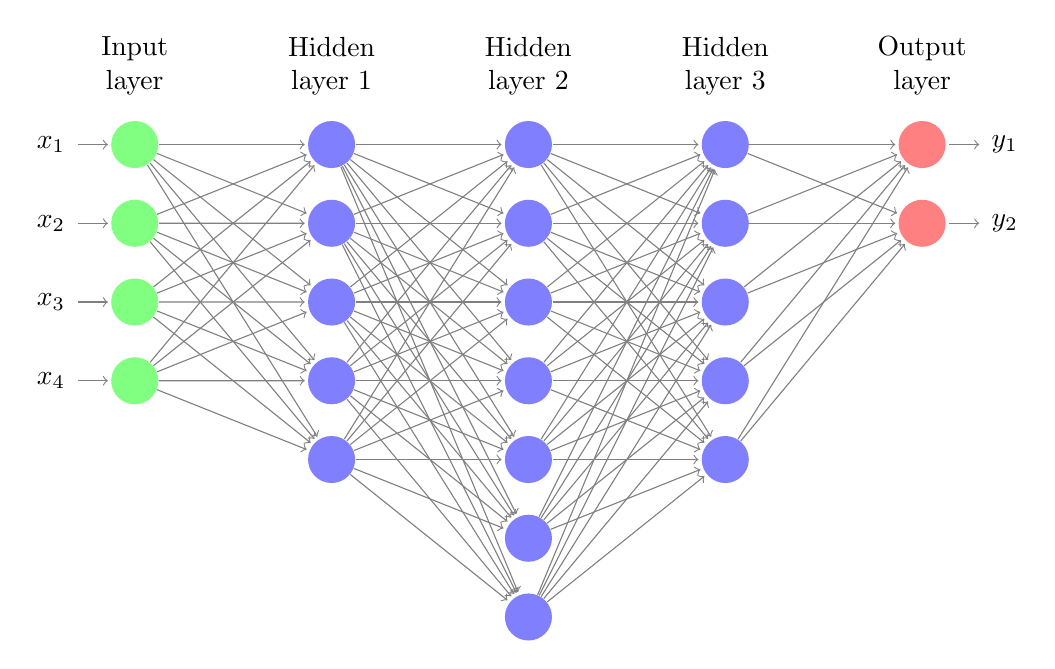
\begin{tikzpicture}[shorten >=1pt,->,draw=black!50, node distance=\layersep]
	\tikzstyle{every pin edge}=[<-,shorten <=1pt]
	\tikzstyle{neuron}=[circle,fill=black!25,minimum size=17pt,inner sep=0pt]
	\tikzstyle{input neuron}=[neuron, fill=green!50];
	\tikzstyle{output neuron}=[neuron, fill=red!50];
	\tikzstyle{hidden neuron}=[neuron, fill=blue!50];
	\tikzstyle{annot} = [text width=4em, text centered]
	
	\pgfmathsetmacro{\nIn}{4}
	\pgfmathsetmacro{\nHa}{5}
	\pgfmathsetmacro{\nHb}{7}
	\pgfmathsetmacro{\nHc}{5}
	\pgfmathsetmacro{\nOut}{2}
	
	% Draw the input layer nodes
	\foreach \name / \y in {1,...,\nIn}
	% This is the same as writing \foreach \name / \y in {1/1,2/2,3/3,4/4}
	\node[input neuron, pin=left:$x_\y$] (I-\name) at (0,-\y) {};
	
	% Draw the hidden layer nodes
	\foreach \name / \y in {1,...,\nHa}
	\path[yshift=0cm]
	node[hidden neuron] (Ha-\name) at (\layersep,-\y cm) {};
	\coordinate (Ha) at (\layersep, \nHa/2 cm );
	
	
	\foreach \name / \y in {1,...,\nHb}
	\path[yshift=0cm]
	node[hidden neuron] (Hb-\name) at (2*\layersep,-\y cm) {};
	\coordinate (NodeHb) at (\layersep, \nHb/2 cm );
	
	\foreach \name / \y in {1,...,\nHc}
	\path[yshift=0cm]
	node[hidden neuron] (Hc-\name) at (3*\layersep,-\y cm) {};
	\coordinate (NodeHc) at (\layersep, \nHc/2 cm );
	
	% Draw the output layer node
	\foreach \name / \y in {1,...,\nOut}{
	\path[yshift=0cm]
	%node[output neuron, pin={[pin edge={->}]right:$y$}, right of=NodeHb] (O-\name) at (3*\layersep,-\y cm) {};
	node[output neuron, pin={[pin edge={->}]right:$y_\name$}, right of=NodeHb] (O-\name) at (3*\layersep,-\y cm) {};
}
%	\node[output neuron,pin={[pin edge={->}]right:y}, right of=H2-3] (O) {};
	
	% Connect every node in the input layer with every node in the
	% hidden layer.
	\foreach \source in {1,...,\nIn}
	\foreach \dest in {1,...,\nHa}
	\path (I-\source) edge (Ha-\dest);

	\foreach \source in {1,...,\nHa}
	\foreach \dest in {1,...,\nHb}	
	\path (Ha-\source) edge (Hb-\dest);
	
	% Connect every node in the hidden layer with the output layer
	\foreach \source in {1,...,\nHb}
	\foreach \dest in {1,...,\nHc}
	\path (Hb-\source) edge (Hc-\dest);
	
	\foreach \source in {1,...,\nHc}
	\foreach \dest in {1,...,\nOut}
	\path (Hc-\source) edge (O-\dest);
	
	
	% Annotate the layers
	\node[annot,above of=Ha-1, node distance=1cm] (hl) {Hidden layer 1};
	\node[annot,above of=Hb-1, node distance=1cm] (hl) {Hidden layer 2};
	\node[annot,above of=Hc-1, node distance=1cm] (hl) {Hidden layer 3};
	\node[annot,above of=I-1, node distance=1cm] {Input layer};
	\node[annot,above of=O-1, node distance=1cm] {Output layer};
	%\node[annot,below of=I-\nIn, node distance=1cm] {$\mathbf{x}$};
	%\node[annot,below of=O-\nOut, node distance=1cm] {$\mathbf{y}$};
	
	\end{tikzpicture}
	
	
\end{document}